\chapter{绪论}
\section{研究背景}
直升机可垂直起降、定点悬停,外带吊挂运输飞行时不受地理地形、货物外形、体积等约束,在军民两方面均取得广泛应用。但目前在国民经济建设过程和应急抢险中涉及到重型载荷运输时,只能租借、购买国外先进国家的直升机执行吊挂飞行任务,一是因为我国重型直升机较少,二是直升机带吊挂飞行时,直升机与吊挂物存在运动耦合,往往会导致直升机飞行品质降低、飞行包线缩小,系统运动振荡发散时还会给直升机带来飞行安全威胁。而国内在直升机带吊挂系统飞行所涉及的飞行力学建模、动力学特性分析、飞行品质、飞行控制等关键技术领域还存在较大不足,与国外相比仍有较大差距。

目前解决重型物资的运输问题,研究工作主要集中在:(1)研制重型直升机,但体积重量的增加,会导致其研制复杂性成倍增加,当直升机运载能力超过一定范围后,直升机性能和经济性也会显著降低[1,2];(2)采用多直升机协同吊挂运输重型载荷[3]。相比重型直升机研制,多直升机协同吊挂具有经济优势,但也同样面临系统运动耦合强、飞行品质低等问题,以及多机干涉、多机交互、环境不确定性等新增问题。考虑到重型直升机研制代价、周期、技术可行性,多直升机协同吊挂作为重型载荷运输的可替代方案,已成为当前研究的热点,这也是本课题的研究方向。

多直升机协同吊挂系统主要由多个直升机、吊挂物、吊挂绳索三部分组成。在多机协同吊挂任务中,吊挂物一般体积大、质量重,甚至在电力巡线、战场空投等任务中具有一定的方向性,不宜再像以往许多研究中当作质点处理,而应考虑其飞行姿态、轨迹,保障多机吊挂运输任务的顺利完成。吊挂物通过绳索与多个直升机相连,多机协同吊挂系统通过控制直升机的运动改变吊挂物的姿态、轨迹。而直升机的运动在满足吊挂物的姿态、轨迹任务需求的同时,还应充分考虑本机飞行性能限制、飞行品质要求、各直升机的差异、与相邻直升机的距离、外界环境等。三个以上直升机协同吊挂时还存在操纵冗余的问题,如何实现协同吊挂任务的最优分配也是当前的研究热点之一。此外,多直升机交互过程中,由于传感器误差、外界环境不确定性等的影响,直升机获得的态势信息往往具有不确定性,这也给多机协同吊挂系统飞行品质带来了巨大挑战。由此可见,如何采取合理策略,充分考虑吊挂任务需求、操纵冗余、环境不确定性、多机交互、各机差异等问题,提高多直升机协同吊挂系统飞行品质,保障多机运输任务顺利完成,值得深入研究。

模型预测控制可以很好地实时处理系统状态、控制、输出约束、环境不确定性等,近年来在无人机控制律设计、编队飞行控制领域取得了广泛应用,这为多直升机协同吊挂中直升机控制技术的设计提供了有效手段。同时,考虑到直升机协同吊挂系统的耦合性,不能简单地将模型预测控制生搬硬套,而应在充分考虑系统特性的基础上对模型预测控制加以改进,以适应直升机协同吊挂飞行需求。

此外,如何综合考虑各直升机性能差异、约束等,计算出吊挂物实现既定轨迹时,所需吊索提供的力及各直升机的位置,也是一大难题。合作微分博弈论可以在充分考虑多智能体间差异性的同时使系统目标最优,为解决上述问题提供了新思路。

本课题以提高直升机协同吊挂运输时的飞行品质和飞行安全为目标,针对直升机协同吊挂运输飞行时的控制技术开展深入研究。旨在建立扩展性强、可考虑气动干扰的多直升机吊挂系统动力学模型,分析直升机协同吊挂系统的操稳特性;综合考虑系统误差、环境不确定性、多机干涉等因素,提出基于改进模型预测控制的直升机控制技术;充分考虑各直升机性能差异、约束等,提出基于合作微分博弈的吊挂系统控制策略;在上述基础上,形成以吊挂物为主导的分层控制技术,完成直升机协同吊挂系统轨迹跟踪、特情应对仿真,及相应的试飞试验。

\section{国内外相关技术研究现状}
\subsection{直升机带吊挂系统飞行动力学建模及特性}
带吊挂物系统动力学建模及特性主要包括吊挂系统建模、直升机带吊挂系统耦合建模、带吊挂系统耦合特性分析三部分。
\subsubsection{吊挂系统建模}
吊挂系统一般包括吊挂物、吊索,以及一些辅助增稳飞行的装置:支撑杆[4-6]、主动臂[7]、尾鳍[8,9]、风速杯[10]、吊索滑轮[11]、可移动吊钩[12-14]等。本节仅讨论这些辅助装置的建模方法,其对带吊挂飞行的控制增稳作用放在带吊挂控制技术一节中讨论。

国外吊挂物建模开始较早,经历了由简单到复杂的过程。早期动力学建模[15-17]及一些吊挂飞行控制技术研究[18-22]中往往将吊挂物当作质点处理,忽略了吊挂物气动载荷的作用。这虽然简单,但不能模拟前飞时吊挂物的后摆运动。随后出现的吊挂物准定常气动阻力模型,将吊挂物气动阻力通过阻力系数、等效迎风面积、当地动压的乘积来表征。这可以反映吊挂物的后摆运动,也简单易行,因此得到了广泛应用[23-28]。但吊挂物具有一定的体积,不仅仅具有阻力,因此随着风洞试验及计算流体力学(CFD)技术的发展,越来越多的研究关注吊挂物的六力素,将吊挂物当作六自由度刚体处理。Szustak[29]首次公开了军用可拆卸集装箱MILVAN(8×8×20英尺)的风洞试验数据,并指出其非线性不稳定气动力矩会对吊挂飞行产生不利影响。随后较多研究[30-34]根据风洞试验或理论数据建立了吊挂物的经验公式气动模型、非线性插值模型等。这些模型计入了吊挂物的六力素,不再仅仅考虑吊挂物的阻力,一般被称为吊挂物准定常气动模型。后来在UH-60A直升机携带军用集装箱CONEX(6×6×8英尺)吊挂飞行过程中发现,当飞行速度超过60节时,由于吊挂物不稳定性,直升机无法继续加速,而此时的飞行速度远远小于UH-60A直升机的最大飞行速度120节[35]。这与采用准定常吊挂物气动模型得到的结论不符,进而引起了多数学者对吊挂物非定常气动载荷的关注。理论结果及风洞试验发现吊挂物非定常气动载荷主要是由非定常气动偏航阻尼引起的。进而,越来越多的研究[36-43]针对吊挂物的偏航气动载荷,建立了航向非定常气动模型。至今,吊挂物的非定常气动建模仍是当前的研究热点。

吊索建模包括刚性、柔性两种。刚性吊索假设绳索长度不变,即直升机与吊挂物吊挂点之间的距离不变[44-46]。弹性绳索建模包括只考虑弹性[47,48],考虑弹性及阻尼[33,34,49,50],同时考虑弹性、阻尼、吊索质量、吊索气动力[51]等。针对辅助装置建模,支撑杆一般被建模为刚体和无质量二力杆[52-54],主动臂、尾鳍、风速杯一般采用CFD方法分析设计以增加吊挂物的航向稳定性[7-10],吊索滑轮、可移动吊钩一般采用传递函数的方式开展建模[11-14]。

国内针对吊挂系统建模起步较晚。针对吊挂物建模主要包括当作质点处理[55,56]、准定常气动阻力模型[57-66]、准定常气动模型[67-70]等手段,较少涉及非定常气动建模。吊索模型的建立涉及刚性、柔性两种。针对辅助装置,马超[71]等采用CFD方法计算了附加尾鳍对吊挂飞行中航向稳定性的作用,并提出了一种直升机吊挂尾鳍尺寸设计方法。针对其他辅助装置的研究较少。

\subsubsection{直升机带吊挂系统耦合建模}
与吊挂物气动建模发展过程类似,直升机带吊挂系统耦合建模也经历了由简单到复杂的过程。Lucassen 等[15]针对直升机吊挂飞行悬停状态建立了平面内的两自由度直升机模型;吊挂系统仅包括连接于吊挂点处的单自由度刚体吊挂物模型。吊挂点处的一对作用力和反作用力分别对直升机和吊挂系统的作用形成了吊挂系统和直升机的相互耦合。Dukes[16,17]在直升机吊挂飞行研究中建立了类似的直升机模型,吊挂系统由单根刚性吊索和质点吊挂物组成。Sridharan等[72]在 Lucassen 等[15]的基础上用气动导数描述直升机模型,并在吊挂飞行中得到了广泛应用[73~81]。

随着直升机飞行动力学建模研究的发展,一些相对复杂的非线性直升机模型[82~85]开始用于直升机吊挂飞行动力学建模研究中,这些模型中不仅包含了旋翼的桨叶动力学模型和入流模型,而且包含了其余各部件的气动模型、机体六自由度动力学模型及各部件间的气动干扰。与此同时,吊挂系统和直升机的耦合建模中也开始考虑旋翼尾流对吊挂物的干扰建模。在 Briczinski 等[48]的直升机吊挂飞行研究中,将小速度状态下直升机旋翼尾流对吊挂物的下洗直接等效为吊挂物额外受到的垂向载荷。在 Shaughnessy 等[31]的模型中,吊挂物的垂向空速中引入了 9.14m/s 的定常速度修正项用于描述旋翼下洗的影响。为了更准确地描述气动干扰的边界和强度的变化,Guglieri 等[86]根据旋翼尾迹发展的特点建立了相似的旋翼尾迹经验模型,针对不同的飞行状态通过吊挂物相对于旋翼桨毂中心的位置判断吊挂物是否处于尾迹当中以及受到多强的干扰。

\subsubsection{带吊挂系统耦合动力学特性分析}
关于带吊挂系统的耦合动力学特性分析,主要体现在带吊挂飞行时直升机、吊挂物的稳定性及模态变化上。针对单机吊挂,Briczinski等[48]分析了吊索刚度对直升机吊挂飞行系统垂向颠簸模态(Vertical bounce mode)稳定性的影响。研究指出吊索刚度越大,伸长量越小,稳定性越好。同时由于直升机一般具有较大的垂向阻尼,该模型稳定性较好。Gera 等[4]分析了吊索长度、吊挂物质量、吊挂物回转半径、空气密度以及前飞速度对吊挂系统横向摆动模态和吊挂物航向模态稳定性的影响。Poli 等[30,87]分析了吊索长度以及吊挂物气动阻力与重力比对吊挂系统运动模态稳定性的影响。Nonnenmacher 等[88]分析了吊点位置、吊索长度和吊挂物质量对吊挂系统运动模态稳定性的影响。除了吊挂系统的运动模态,包括直升机运动模态在内的吊挂飞行的运动模态也备受关注。Stuckey[89]分析了飞行速度和吊挂物质量对吊挂飞行运动模态稳定性的影响。Lucassen 等[15]分析了吊挂点相对直升机重心的位置、吊挂物质量以及吊挂物重心到吊挂点的距离对吊挂飞行运动模态稳定性的影响。Dukes[16,17]分析了吊索长度和吊挂物质量对稳定性的影响。Guglieri 等[46,86]分析了前飞速度、转弯速率、吊挂物质量、吊挂物等效阻力面积以及吊索长度对稳定性的影响。Oktay 等[90]分析了吊挂物质量、吊挂物等效平板面积以及吊索长度对稳定性的影响。单直升机带吊挂飞行的动力学特性为多机吊挂动力学特性的研究奠定了基础。

针对多机吊挂,Curtiss等[2]开展了双直升机带支撑杆吊挂悬停时,支撑杆、绳子形状不同时的动力学特性分析工作。Raz等[91]开展了双直升机带支撑杆吊挂前飞时的动力学特性分析工作,研究表明在整个飞行包线内,双机带吊挂系统均存在不稳定模态。Cicolani等[5]指出双直升机带支撑杆吊挂稳定飞行时,吊挂物、支撑杆上的吊挂点必须在同一竖直平面内。双机吊挂的另一种形式是不带支撑杆吊挂,具有结构简单、飞行阻力小的优点,但由于没有支撑杆,悬停时直升机需要有一定的滚转角,也需要更长的吊索来避免直升机间的碰撞[3]。驾驶员在评价不带支撑杆吊挂时认为悬停时直升机姿态角过大,驾驶员工作负荷过大,不利于吊挂飞行,对这种吊挂方式的研究较少。无人直升机的出现使上述问题得以解决。Berrios等[22]开展了双自动R-MAX直升机不带支撑杆吊挂的研究,并指出存在一个影响姿态响应的双升力模态(dual lift mode),在内环控制律设计时需要加以考虑。 

国内相关学者也对带吊挂系统的耦合动力学特性作了分析。针对单机吊挂,崔瑛[57]、陈元[92]研究了不同吊挂物重量、不同吊索长度、不同前飞速度对直升机和吊挂物运动模态的影响。曹义华团队[61-66,69-71]分析了吊挂参数改变对直升机稳定性的影响,给出了直升机带吊挂飞行时的响应特性分析,并基于ADS-33对直升机带吊挂系统悬停飞行品质作了研究。针对多机吊挂的研究较少。宋彦国[93]研究了多直升机带吊挂系统的耦合动力学特性,并明确指出多直升机协调吊挂系统中每一架直升机均具有不同的稳定性与响应形式。

以上研究结果均表明:直升机带吊挂飞行时,由于存在耦合,对直升机和吊挂物的稳定性均产生了不同程度的影响(具体影响程度取决于吊挂物重量、吊挂点位置、吊索长度、吊挂物模型等因素)。运动模态的稳定性是飞行品质评价的重要指标,对控制律的设计具有重要指导意义,值得深入研究。

\subsection{带吊挂系统控制技术}
\subsubsection{单直升机带吊挂控制技术}
单直升机带吊挂控制技术包括被动控制和主动控制两种。关于直升机带吊挂飞行被动控制技术,Smith为了在不过多增加系统功率的基础上增加负载阻尼,设计了主动臂来抑制吊挂物的震动,并开展了相关的试飞试验。Gera[4],Cicolani[8],Raz[9]增加了尾鳍来提高吊挂物的航向阻尼。针对UH-60A直升机携带军用集装箱CONEX(6×6×8英尺)吊挂飞行,文献[8]表明通过增加尾鳍的方式可以将带吊挂飞行最大速度由60knots增加到110knots。文献[10]表明,通过在吊挂物上增加风速杯,UH-60A携带CONEX带吊挂飞行最大速度可以增加到120knots。国内相关研究开展较晚,马超[71]等采用CFD方法计算了附加尾鳍对吊挂飞行中航向稳定性的作用,并提出了一种直升机吊挂尾鳍尺寸设计方法,几乎没有文献提及其它被动控制技术。值得注意的是,通过在吊挂物上增加辅助装置来抑制吊挂物摆动的方式虽然效果显著,但针对不同的吊挂物辅助装置需要重新设计。此外,辅助装置还会增加吊挂物的重量。

关于直升机带吊挂飞行主动控制技术,Asseo[11]针对重型直升机带吊挂飞行稳定性作了控制设计,研究表明带吊索滑轮的三点吊挂方式可以更好地抑制吊挂物振荡。Patterson[12]、Enciu[13]、Singh[14]等设计了可移动的货物挂钩,实现了直升机带吊挂物全飞行包线飞行。Le[94]、Park[95]等通过可变吊索长度的方式实现了吊挂物的线性控制。上述主动控制技术与被动控制技术类似,均存在吊挂物重量增加的问题。主动控制技术的另一种方式是反馈吊挂物摆角到直升机飞行控制中,通过直升机的运动来抑制吊挂物振荡。Ivler等[96,97]的研究表明通过反馈吊挂物摆角/角速度到直升机飞行控制中,可以提高直升机带吊挂飞行控制系统的操纵品质。随后,文献[98]针对直升机带吊挂低速飞行时,采用反馈吊挂物摆角的方式,开展了相关试飞试验工作,试验表明反馈吊挂物摆角有利于抑制吊挂物振荡。Bisgaard[99-102]对直升机带吊挂飞行控制技术的研究做了很多工作:首先开展了单/多直升机带吊挂系统的建模,接着依次提出了输入整形技术、延迟反馈吊挂物摆角控制来抑制吊挂物的振荡,最后将上述两种策略与直升机原有飞行控制结合,实现了直升机带吊挂飞行的自主控制技术。Omar[103]、Krishnamurthi[104,105]、Sonobe[106]也采用延迟吊挂物摆角反馈技术设计了直升机带吊挂飞行的控制,并开展了仿真验证工作。Haviland[107]等针对无人直升机带吊挂飞行,基于期望吊挂物轨迹,设计了自适应动态逆控制器来控制直升机运动,利用一个前置摄像头估计吊挂物的位置,相关仿真及试验验证了此控制律的有效性。la等[108]基于最优控制设计了直升机带吊挂飞行的控制律,Omar等[109,110]基于模糊控制设计了抑制吊挂物摆动控制律。Scaramal[111]等在反馈吊挂物摆角的基础上,基于飞行速度设计了任务调度控制器,仿真结果表明采用上述控制律带CONEX集装箱飞行时速度可以提升到130knots。如何设计有效控制律抑制直升机带吊挂系统耦合振荡,实现直升机带吊挂全包线飞行,仍是当前研究热点。

国内对于直升机带吊挂飞行控制的研究起步较晚,但也取得了一定成果。王海宁[112,113]根据系统固有频率和阻尼,设计了基于指令光滑技术的控制器,有效抑制直升机吊挂系统中负载和直升机速度的振荡,仿真和实验证明了上述控制算法的有效性。毕梦月[114]基于PID控制方法设计了一套能够改善直升机/吊挂物耦合系统操稳特性的飞行控制律并进行了仿真验证。戴勇[115]等在成熟的无人直升机控制律基础上,使用了输入整形前馈控制和缆位角反馈控制方法来抑制缆绳振荡,仿真结果证明了该方法的有效性。但上述研究中吊挂物建模采用质点模型[112,113,115],或者准定常气动模型[114],没有计入吊挂物的非定常载荷,不能反映直升机带吊挂物较大速度前飞时的控制问题,具有一定的局限性。

\subsubsection{多直升机带吊挂控制技术}
单直升机吊挂控制中为多直升机吊挂控制奠定了基础。Curtiss[2]研究了双CH-54直升机带支撑杆吊挂的控制策略,并指出支撑杆带来的额外重量会增加驾驶员的工作负载。Rodriguez[18]提出了双直升机带支撑杆吊挂系统多变量集中式自动飞行控制方案。Mittal等[74]研究了具有不确定性参数的双直升机带吊挂系统的跟踪控制问题,设计了自适应反馈控制律来估计系统的不确定性,仿真验证了控制律的有效性。Menon等[116]设计了双直升机带吊挂系统非线性控制律,仿真结果验证了控制律的性能,分析了参数敏感性。Reynolds等[117]对两架US-60A黑鹰直升机带负载飞行,以控制量和俯仰运动最小为目标,针对不同的吊索长度设计了控制律,仿真验证了控制律的可行性。Bernar等[21,80]等开展了三个小型直升机协同吊挂的控制策略研究,考虑整个系统(三个直升机和一个吊挂物)的动态,设计了内外环控制器,并在吊索上布置力传感器反馈到内环控制器中提高系统鲁棒性,仿真和试验试飞验证了控制律的可行性,这也是全球范围内首次三架直升机协同吊挂运输的演示试验。Li等[118]针对四直升机协同吊挂系统提出了分层控制策略:首先根据吊挂物目标轨迹计算吊挂物运动所需的合力、合力矩,然后由合力、合力矩计算需要每根吊索提供的力,最后根据每根吊索的力和长度计算每个直升机的目标位置。上述研究还指出四个直升机协同吊挂时存在操纵冗余问题。Berrios[22]等设计了两架无人R-MAX直升机带吊挂的控制策略:设计了考虑不稳定双升力模态的角度环控制器,指出相比单机吊挂中包含两个钟摆模态,双机吊挂中仅包含一个钟摆模态,并采用多目标参数优化方法优化控制器参数,仿真结果表明该系统可以满足ADS-33E稳定性和飞行性能要求。Takahashi[116]等利用两架Yamaha R-MAX直升机开展了起飞、着陆、5m/s前飞试验,并指出采用吊挂物摆角反馈控制可以增加悬停时吊挂物的阻尼。Enciu等[120]针对四直升机带吊挂系统,在无需吊索力和吊挂物状态反馈的基础上,设计了动态逆控制律来增加系统稳定性、保障机动飞行时编队形状的稳定,并指出可以优化四直升机协同吊挂系统编队形状以提高性能和飞行品质。国内针对多机吊挂控制的文献较少。宋彦国等[121,122]基于直升机控制输入逆解的方法,研究了多直升机吊挂系统的控制问题,并指出该方法能直接处理吊索力反馈,保证多直升机吊挂系统中每一架直升机具有相同的控制律并能有效抑制吊索力扰动,仿真结果证明了该方法的可行性和正确性。

上述文献为多直升机带吊挂控制的研究奠定了基础,但均没有考虑各直升机性能差异、环境不确定性、多机交互等问题,在综合考虑多方因素,提高系统飞行品质方面,仍具有较大的发展空间,这也是本文的主要研究目的。

\subsubsection{多轴无人机带吊挂控制技术}
由于多轴无人机结构简单、代价低廉、试飞试验易于开展,近年来许多学者也开始关注多轴无人机带吊挂的控制技术,这也给直升机带吊挂技术的研究提供了借鉴。针对单个多轴无人机带吊挂,Sadr等[123]将吊挂物当作质点,基于牛顿-欧拉方程建立了单个四旋翼带吊挂的八自由度动力学模型,然后在上述非线性模型的基础上,设计了抑制吊挂物振荡控制律,仿真证明了上述策略的有效性。Dai等[124]针对吊挂物重量不确定时的单四旋翼带吊挂作了研究,设计了固定增益PD控制器,并提出了一种自适应控制策略来补偿吊挂物重量带来的不确定性。Trachte等[125]为单个四旋翼带吊挂系统设计了带约束的非线性模型预测控制器,仿真表明该控制律不仅可以控制四旋翼按给定轨迹运动,还可以抑制吊挂物摆动,与线性二次最优控制器相比效果更优。Kui等[126]指出吊挂物的存在会降低四旋翼的控制性能,随后针对四旋翼带吊挂系统设计了滑模控制器,仿真结果表明了控制策略的可行性。Shi等[127]指出吊挂物的钟摆运动会改变四旋翼的动力学特性,并在控制律设计过程中将吊挂物运动当作扰动处理,并基于谐波扩展状态观测器设计了高精度扰动补偿器,仿真及试验表明了上述策略在四旋翼吊挂飞行时的鲁棒性。Yu等[128]针对四旋翼带吊挂飞行,设计了非线性反演控制器,并开展了相关试验。Yi等[129]等在不改变四旋翼原本控制律结构和参数的基础上,设计了卡尔曼滤波器来估计由吊挂物运动带来的不确定性,并集成到原本的控制器中,基于pixhawk的四旋翼带吊挂试验平台验证了上述控制律的有效性。Cabecinhas等[130]为四旋翼带吊挂系统设计了轨迹跟踪控制器,并开展了仿真验证和试验试飞工作。Wang等[131]针对四旋翼带吊挂系统,设计了双精度自抗扰控制器,将吊挂物运动和外界环境不确定性当作扰动处理,并利用非线性状态扩张观测器进行在线估计,试验结果验证了上述控制律的有效性。

针对多个多轴无人机带吊挂飞行,Yoo等[132]基于Udwadia-Kalaba方程开展了多个四旋翼无人机协同运输系统的建模,还进行了稳定性分析和简单的控制律设计。Lee等[133-135]作了较多工作:通过球面坐标-牛顿法建立了带吊挂系统的动力学模型,采用线性二次高斯/环路转移恢复(Linear quadratic Gaussian / loop transfer recovery)的方法控制各无人机、吊挂物的位置、姿态;针对不同重量的吊挂物及不能被原本控制器估计的扰动,设计了参数鲁棒线性二次高斯法以提高稳定性;仿真结果验证了上述控制律的有效性。Aghdam等[136]针对吊挂物重心可移动的四个四旋翼带吊挂飞行开展了控制律设计,通过领导-跟随结构保持队形,采用反馈线性控制器保持四旋翼z轴方向的稳定。Klausen等[137]针对未知吊挂物重量、存在外界环境扰动的多四旋翼无人机带吊挂开展控制律设计及试验试飞工作。Shirani等[137]针对多四旋翼无人机带吊挂飞行,基于分布式控制思想,设计了线性最优控制与PID结合的控制器,在保持队形的同时尽可能减少吊挂物摆动。Geng等[139,140]以吊挂物为主导,设计了多无人机协同吊挂分层控制策略(与文献118类似),并指出四个及以上无人机带吊挂飞行时吊索层存在冗余问题,接着分析了上述问题的非凸性,提出了将非凸性优化问题转换为凸优化的方法,最后开展了仿真验证及试验试飞工作。Ariyibi等[141]等开展了两个四旋翼无人机带吊挂飞行的研究工作,设计了领导-跟随结构来保持队形,采用了队形引导和推力矢量的控制方法,研究表明即使没有对吊索、吊挂物进行建模,双四旋翼带吊挂系统仍能保持队形。Jackson等[142]提出了一种分布式轨迹优化并行计算方法来处理非线性动力学及非凸优化问题,并将其应用到了多四旋翼无人机协同吊挂飞行中。

近年来,国内学者也展开了对多轴无人机带吊挂飞行的研究。鲜斌等[143]通过能量分析的方法设计了四旋翼带吊挂系统的非线性控制器,可以在抑制吊挂负载摆动的同时将四旋翼无人机移动到目标位置。孙冰寒[144]针对四旋翼无人机携带吊挂负载的航迹规划问题,基于预测控制设计了以路线最短、躲避障碍物以及减小负载的摆动为性能指标的代价函数,实现了四旋翼无人机的空间位置实时规划。吴超凡[145]采用拉格朗日动力学对四旋翼吊挂系统进行动态建模,模型以四旋翼机体运动和负载摆动为主体,考虑了四旋翼与负载之间的耦合关系,建立了非线性数学模型。根据两种方式,PD控制和引入滤波器,设计对应的位置控制器和姿态控制器,实现对目标点的轨迹跟踪,并比较了两种方法的优劣。王诗章[146]主要考虑了四旋翼无人机吊挂飞行系统的位置控制及负载摆动抑制的设计问题.在存在欠驱动特性以及未知系统参数的约束下,基于能量法设计了一种非线性控制策略,实现了对无人机位置的精确控制和飞行过程中负载摆动的快速抑制。秦欢[147]利用串级PID控制器,采用分步设计思路对飞行控制系统的姿态回路和轨迹回路控制律进行设计,并对整定后的四旋翼带吊挂飞行控制系统进行飞行试验,从自主起降、高度保持和构件抓取等方面验证飞行控制系统的控制效果。郭民环[148]指出2个四旋翼无人机(UAVs)的吊挂飞行问题属于协同合作的范畴,为了充分利用无人机各自的性能,将其看成是具有不同目标函数的决策主体,并在非合作博弈的框架下进行控制器设计,仿真验证了上述控制律的有效性。
多轴无人机带吊挂飞行控制技术为直升机带吊挂飞行的研究提供了参考,可相比直升机,多旋翼无人机载重能力低、续航时间短。且直升机耦合强、灵敏度低,与多旋翼无人机相比有一定的差异。此外,在多轴无人机带吊挂飞行的多数研究中,均将吊挂物当作质点处理,不能充分反映吊挂物的实际运动状态。因此,针对多直升机带吊挂系统协同控制技术的研究具有更大的难度,也是非常有益和十分必要的。

\subsection{模型预测控制}
模型预测控制近年来被广泛应用于无人机轨迹跟踪、编队飞行中单个无人机控制律设计等领域。其控制机理可以描述为:在每一采样时刻,根据获得的当前测量信息和参考量的差异建立代价函数;通过优化代价函数在线求解一个有限时域开环优化问题,并将得到的控制序列的第一个元素作用于被控对象;在下一个采样时间,重复上述过程。

Wan等[149]建立了无人直升机的六自由度模型,提出了一种基于神经网络反馈控制器和状态相关Riccati方程(SDRE)控制器的组合最优控制方法,神经网络控制器的优化是在模型预测控制的框架内进行的,SDRE提供初始可行的方案来增加神经网络模型预测控制的鲁棒性。

Castillo等[150]提出了一种用于小型无人直升机的基于模型预测控制的轨迹跟踪(MPCTT)系统,并与经典PID实现的速度跟踪和位置跟踪系统进行了比较,仿真结果证明了MPCTT控制方法的优越性。

Joelianto等[151]对小型直升机模型预测控制的可行性作了研究,针对该小型直升机模型从悬停到前飞的五个线性模型作了模型预测控制器设计,结果表明采用模型预测控制,系统具有良好的鲁棒性和轨迹跟踪性能。

Liu等[152]针对无人直升机,设计了一个高级模型预测控制器和一个低级线性控制器。模型预测控制器以分段恒定的方式工作,以减少计算负担并增加可用于执行在线优化的时间。线性反馈控制器可响应直升机的快速动态变化,并补偿高级控制器的低带宽。最后,在小型直升机上进行了仿真和飞行测试,验证了所提控制方案的有效性和可行性。

Yao等[153]基于模型预测控制(MPC)和改进的灰狼优化器(IGWO),提出了一种混合方法来规划城市环境下目标跟踪的多无人机的最优轨迹。

Andrade等[154]采用模型预测控制器来解决倾转旋翼无人飞行器带吊挂飞行时的轨迹跟踪问题:以系统的线性误差作为代价函数,并计入了终端代价来确保模型预测控制器的稳定性,接着在考虑输入和状态约束的同时通过优化计算控制量。

Kamel等[155]研究了无人机模型预测控制设计和实现策略:介绍了多旋翼无人机及固定翼的建模方法,采用系统识别技术计算模型估计值,依据在线优化方法得到控制量。

Cabral等[156]考虑到四旋翼的非线性和欠驱动特性,在各种操作环境下采用了自主学习方法来调整非线性模型预测控制器。具体来说,上述策略应用自主学习方法来选择目标函数的加权参数,以最小化跟踪误差。仿真结果表明,所学习的加权参数可以有效地用于非线性模型预测控制。

Cai等[157]提出了一种事件触发模型预测控制方案用于控制多无人机编队飞行。首先设计了一个分布式模型预测控制框架;接着提出了一种事件触发机制来减少分布式模型预测控制方案的计算负担;然后开发了基于安全距离的禁飞区策略,并将其集成到了代价函数中。数值仿真结果表明,与传统的分布式模型预测控制相比,所提出的事件触发分布式模型预测控制在实现多无人机编队控制方面具有更高的计算效率。

Li等[158]对尾座式无人机悬停时的模型预测控制开展了研究。首先建立了尾座式无人机的动力学模型并将其线性化,然后根据线性化模型设计了模型预测控制器,仿真结果表明设计的模型预测控制器具有良好的轨迹跟踪性能。

Zhihao等[159]提出了一种基于虚拟目标制导的分布式模型预测控制器用于多无人机的编队飞行。首先,设计了一种分布式模型预测控制框架,接着开发了一种虚拟目标制导方法并将其集成到分布式模型预测控制中,以实现轨迹跟踪和避障,然后提出了一种事件触发机制,以减少无人机编队控制的计算负担。数值仿真结果表明了上述控制方案在多无人机编队飞行中的有效性。

Zhang等[160]研究了带有扩展状态观测器的自适应模型预测控制,以应对存在外部干扰和系统不确定性的多无人机编队飞行,并依据Lyapunov稳定性定理分析了所提出的模型预测控制器的稳定性。数值仿真结果证明了所提方案的可行性。


\subsection{吊挂负载分配策略}
直升机可垂直起降、悬停,外带吊挂运输飞行时不受地理地形、货物外形、体积等约束,在军民两方面均取得广泛应用\cite{ronen1985dynamics,cicolani1995simulation,bisgaard2008modeling,bisgaard2010adaptive}。且当前对重型直升机外挂运输的需求愈发迫切,但是体积重量的增加,会导致重型直升机的研制复杂性成倍增加、经济性显著减低,多直升机协同吊挂作为重型直升机运输的一种可替代方案,成为吊挂飞行的研究热点\cite{cicolani1992equations,raz2005trim,yi2018review}。一个系统的能力往往取决于其劣势部分。对于协同吊挂系统,其负载能力及航时航程取决于消耗功率最大的直升机或同等功耗下航时最小的直升机。可见,在考虑各直升机相对位置、性能差异的前提下,合理分配吊挂负载给各个直升机,避免飞行过程中一架或多架直升机过早失效,进而增加整个协同吊挂系统的航时航程,提高其飞行性能,具有重要意义。

目前,较多文献提出了基于吊索拉力相等的负载分配策略。Bernard\cite{bernard2013system}针对两个Yamaha RMAX直升机协同吊挂系统,在各直升机原本自主飞行控制系统的基础上增加了队形变换策略、吊索拉力均等控制、吊挂物摆动抑制控制,完成了仿真验证和飞行试验。Berrios\cite{berrios2018load}设计了一个前馈控制器计算跟随直升机相对主导直升机的位置,同时提出了反馈控制策略使前后直升机受到的吊索拉力相等。结果表明,基于上述负载分配控制器,两个吊索拉力间的差异小于吊挂物重量的2\%。Geng\cite{geng2019implementation,geng2020cooperative}针对四个多轴无人机协同吊挂系统,将整个系统分为吊挂物层、吊索层、直升机层,设置吊索角度、拉力约束,将负载分配问题转换为了吊索拉力凸优化问题,并在此基础上开展了仿真验证和试验试飞工作。Duan\cite{duan2021application}提出采用社会蜘蛛算法求解上述优化问题,鲁棒性高、不易陷入局部最优解。但上述吊索拉力凸优化问题将各个吊索拉力之和最小作为优化目标,不能实现吊索拉力的均等分配。在Geng随后的研究中\cite{geng2020control,geng2021trajectory},基于以吊挂物为主导的分层控制方法,将负载分配问题转化为吊挂物轨迹规划和跟随控制两部分。文章提出了基于直接分配法和强化学习的两种轨迹规划方法,可以实现吊索拉力的均等分配。但吊挂物轨迹的引入会使设计变量成倍增加,导致计算时间长、收敛难度大。

但吊索拉力相等并不能保证各直升机功耗相等。Enciu\cite{enciu2017flight}针对四个UH-60黑鹰直升机协同吊挂运输系统定常平飞状态开展了飞行性能优化研究,指出直升机协同吊挂系统的飞行性能优化问题可以归结为在综合考虑动力学约束、队形约束、安全距离约束的前提下,如何合理分配负载给直升机,以最小化耗能最大的直升机的功率的问题。计算结果表明基于功率消耗的分配策略,前飞速度100 ft/s时,“2-lead”队形的直升机相对基于吊索拉力相等的分配策略最大功耗可降低16 \%。研究指出这是由于基于吊索拉力相等的分配策略,在吊索拉力作用下,前方直升机受到吊索向后的力,相当于额外增加了阻力,直升机需要低头来平衡这部分阻力,功耗增加。反之,后方直升机受到吊索向前的力,直升机抬头,功效减小。基于功耗的分配策略,可以在约束范围内合理调节吊索拉力和角度,使各个直升机功效最小且相等,有利于提高整个系统的飞行性能。然而,上述计算结果仅仅是针对定常平飞状态的,没有给出系统存在机动时的处理方法。此外,文章没有详细给出直升机功率代理模型的计算方法。Song\cite{song2013modeling}给出了类似的结果:针对4个UH-60直升机协同吊挂系统,以各直升机间的距离保持100 ft为约束,开展了不同前飞速度下的配平和稳定性分析工作,计算结果表明随着飞行速度的增加,前方直升机总距需求量远远大于后方直升机。

进一步,针对吊挂物的跟随控制,以往多数文献中往往假设参与协同吊挂的各直升机控制需求相同,或将参与协同吊挂的无人机目标函数简单加权相加作为系统的整体目标函数,没有详细考虑各直升机间的配置差异,也不能引入直升机间互动的影响。Geng\cite{geng2020control,geng2021trajectory}以系统状态量误差和各直升机操纵量之和最小为系统目标,基于Bryson后向扫描法设计了吊挂物跟随控制策略。Gimenez\cite{gimenez2020control}针对带支撑杆的双直升机协同吊挂系统,设计了轨迹跟踪控制目标、避障控制目标、安全距离控制目标等,并通过对上述目标加权基于零空间理论得到了系统控制策略。Arab\cite{arab2021planning}将吊索拉力当作无人机扰动,提出了基于无主导分布式控制的协同吊挂系统控制方法,该方法不能考虑直升机间互动的影响,也不能控制吊挂物位置、姿态等。Chopra\cite{chopra2022distributed}在吊挂物上装载了惯性传感器和光学传感器,以控制吊挂物轨迹和姿态为目标,基于分布式理论设计了控制策略,但该方法不能考虑直升机间的性能差异。

目前,博弈控制已广泛应用到多智能体领域。Jimenez-Lizarraga\cite{jimenez2018differential}首先基于牛顿-欧拉公式,给出了系统的动力学模型,然后提出了一种基于微分博弈方法的n个四旋翼无人机编队飞行控制算法。Jiang\cite{jiang2020cooperative}提出了一种基于合作微分博弈的共享信息多无人机编队飞行控制策略。首先将多无人机编队飞行定义为轨迹跟踪问题,然后基于合作博弈策略,设计了各无人机的代价函数。仿真结果表明了合作微分博弈相比非合作博弈和一般最优控制在无人机编队飞行中的优越性。Chai\cite{chai2020robust}提出了事件触发型鲁棒微分博弈失效卫星接管控制策略,其中各个体通过局部性能指标函数的优化获得控制策略,可以在抵抗外界干扰的同时,实现失效卫星的接管。可见,在博弈控制框架下,各个智能体可以根据自身性能差异和任务不同,在考虑互动影响的前提下,独立设计不同的目标函数。这给本文提出基于微分博弈的抗干扰负载分配策略带来了灵感。

\subsection{微分博弈技术}
微分博弈可以充分考虑各智能体间的差异,在多智能体控制领域取得了显著成果。

Han等[161]针对具有模型不确定性和未知外部扰动的智能体,提出了一种用于多智能体系统无领导者编队的线性二次微分博弈方法。外部干扰被视为虚构的参与者,并在考虑模型不确定性的基础上给出了智能体的代价策略。最后,给出了三角形编队飞行仿真示例,验证了所提方案的可行性。

Jimenez-Lizarraga等[162]提出了一种基于微分博弈方法的n个四旋翼无人机编队飞行控制算法。首先基于牛顿-欧拉公式,给出了系统的动力学模型,然后提出了基于博弈方法的编队飞行方案。数值仿真说明了编队飞行方法的有效性。

Jiang等[163]提出了一种基于合作微分博弈的共享信息多无人机编队飞行控制策略。首先共享信息将多无人机编队飞行定义为轨迹跟踪问题。然后基于合作博弈策略,设计了各无人机的代价函数。仿真结果表明了合作微分博弈相比非合作博弈和一般最优控制在无人机编队飞行中的优越性。

Li等[164,165]研究了多智能体系统的最优编队控制问题。在局部信息条件下,将n个智能体的行为建模为有限水平的非合作差分博弈问题,并研究其Nash均衡解。通过设计个人代价和网络拓扑,实现了规则的多边形编队,避免了智能体之间的碰撞。最后,在二维和三维欧氏空间中进行了数值仿真,证明了所提方法的有效性和可行性。
西北工业大学的罗建军团队[166-170]基于微分博弈研究了多微卫星姿态接管失效航天器的控制方法。罗建军[166]提出了一种基于事件触发鲁棒微分博弈控制的多微卫星姿态接管失效航天器方法,针对贴附在失效航天器表面的多颗微卫星和失效航天器形成的组合体,将存在干扰的姿态接管控制问题建模为多颗微卫星以及干扰之间的博弈问题,避免了控制的分配,并有效抑制了干扰。柴源[167,168]针对多微卫星姿态接管失效航天器问题,提出了状态相关黎卡提方程微分博弈控制方法,通过引入状态相关系数矩阵,将非线性博弈转化为状态相关线性二次型博弈,然后通过李雅普诺夫迭代法求解耦合状态相关黎卡提方程组得到了微卫星的状态反馈控制器,实现了微卫星的自主决策.数值仿真验证了多颗微卫星状态相关黎卡提方程微分博弈控制方法实现姿态接管的有效性和容错性。韩楠提出了失效卫星姿态管接的微分博弈学习控制方法[169]和并行学习合作博弈策略[170]。在微分博弈学习控制方法中,给出了微小卫星微分博弈的HJ (Hamilton-Jacobi)方程,并通过基于单神经网络的策略迭代算法进行了耦合HJ方程解的学习,实现了对微小卫星博弈均衡策略的逼近。在并行学习合作博弈策略中,通过过去与当前时刻数据的并行使用,设计了基于并行学习的策略迭代方法,放松了神经网络权值矢量学习对持续激励条件的要求,给出了为确保神经网络权值矢量估值收敛,所使用的过去时刻数据所需满足的条件,并通过拉格朗日方法分析了神经网络权值矢量估计误差的一致最终有界性。然后采用并行学习策略迭代方法进行了微小卫星合作博弈帕累托最优策略数值解的逼近,实现了多微卫星姿态接管失效航天器的闭环协同控制。

谢剑[171]开展了基于微分博弈论的多无人机追逃协同机动技术研究:建立了双机编队采用微分博弈法对单一无人机进行追捕的机动决策模型;运用几何原理对多无人机编队进行机动飞行控制,使用梯度迭代方法进行模型求解,使得追逃微分博弈论最优机动决策算法能够在多无人机编队中进行使用。仿真结果表明,设计的微分博弈算法能够使得多无人机快速捕获单一目标机,并且能够实现无人机在作战对抗中编队飞行,具有一定的实用价值。

\subsection{协同吊挂系统避障技术}

\section{本文研究对象}

\begin{figure}[!htb]  
  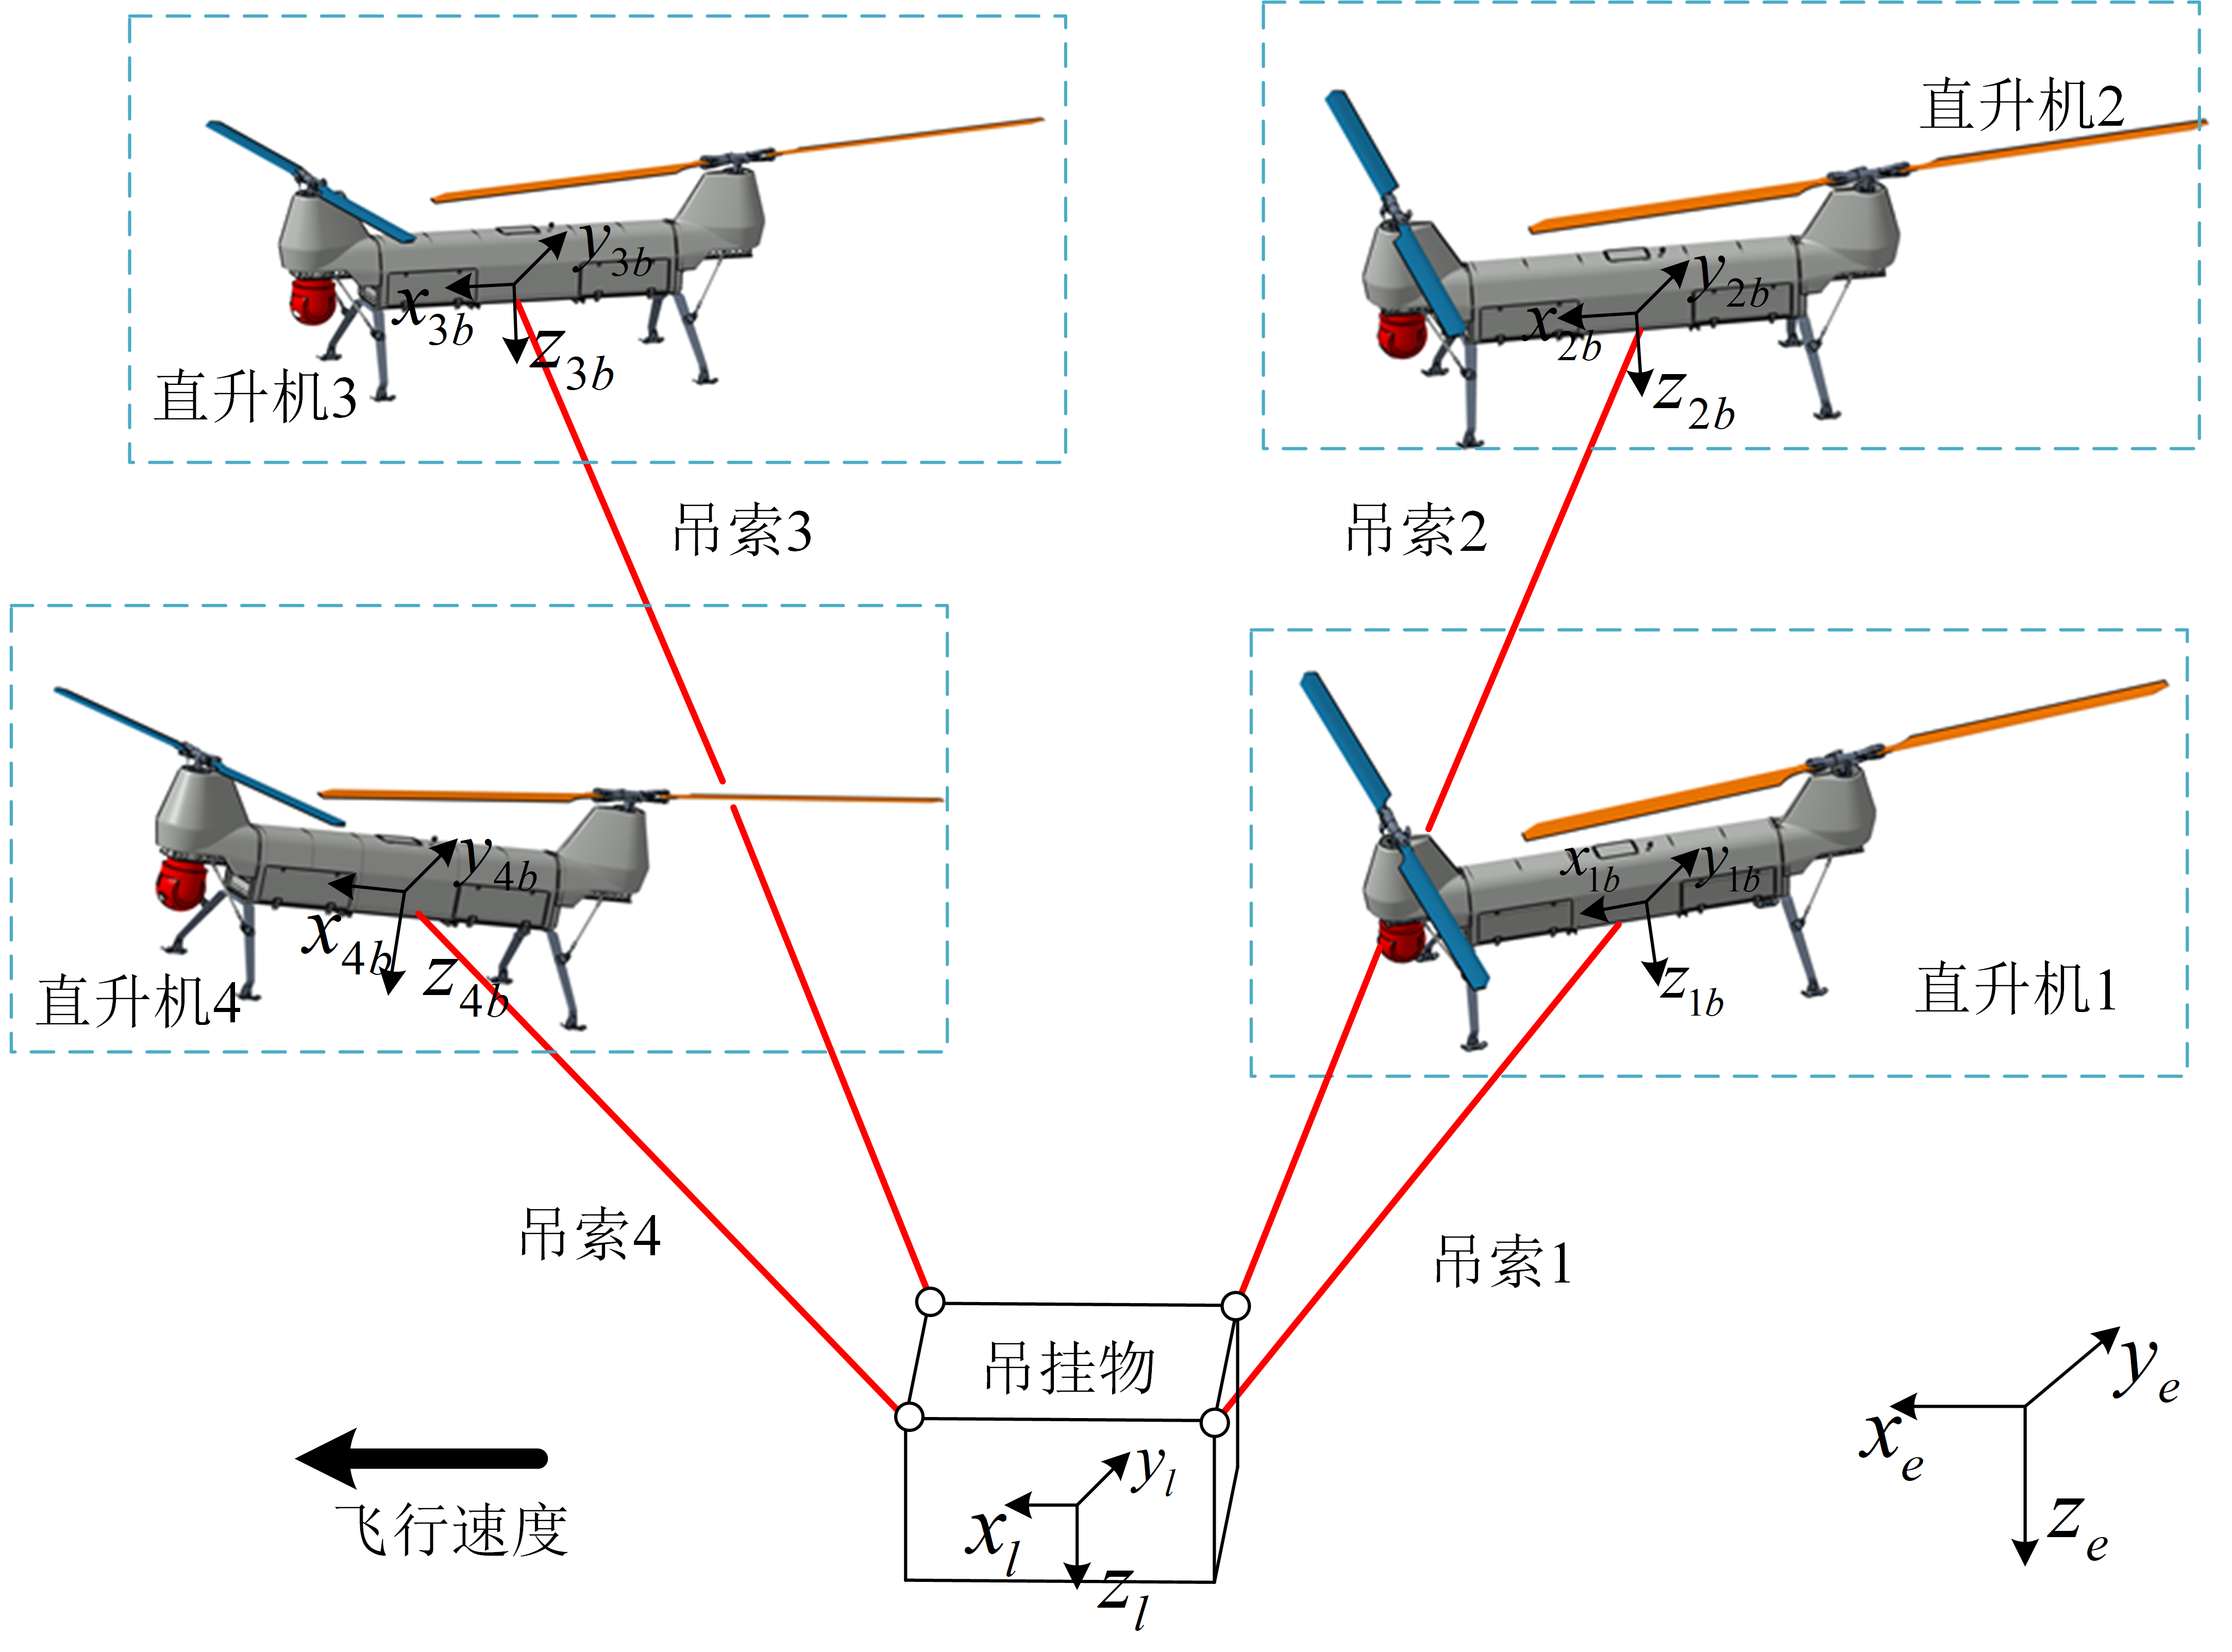
\includegraphics[width=10cm]{fig/figure_chap4/Chap4_1_2.png}
  \caption{本文研究对象:四纵列式直升机协同吊挂系统}
  \label{fig:4_1_2}
\end{figure}

本文研究的是“2-lead”队形的协同吊挂系统。见图\ref{fig:4_1_2},四个纵列式直升机各自采用7.2 m长的吊索协同吊挂负载。每个纵列式直升机有两副两片桨叶的旋翼,旋翼轴间的纵向距离为1.165 m,横向、垂向距离为0。旋翼旋转速度为113 rad/s,直径为1.8 m。负载是长方形的,其长、宽、高分别为1 m,0.4 m,0.4m。其重量为10 kg,大于单个直升机的运载能力(3.5 kg),小于整个协同吊挂系统的运载能力(14 kg)。此外,图\ref{fig:4_1_2}中,$x_ey_ez_e$、$x_{ib}y_{ib}z_{ib}$、$x_Ly_Lz_L$分别代表北-东-地的大地坐标系、直升机$i$的体轴系、吊挂物体轴系。

各个小型纵列式直升机的基本配置参数见下表。
\begin{table}[htb!]
  \caption{纵列式直升机基本配置参数}
  \begin{tabular}{cc}
    \toprule
    项目 & 数值 \\ 
    \midrule
    起飞重量(kg)& 15.0\\
    $I_{xx}\ (\rm{kg \cdot m^2})$ & 0.284 \\
    $I_{yy}\ (\rm{kg \cdot m^2})$ & 2.065 \\
    $I_{zz}\ (\rm{kg \cdot m^2})$ & 2.083 \\
    旋翼半径(m)& 0.9 \\
    桨叶弦长(m)& 0.069\\
    桨叶负扭( \degree )& 0\\
    桨叶片数 & 2\\
    旋翼转速(rad/s) & 113.1 \\
    前侧旋翼相对重心相对位置 & [0.5825, 0, -0.25]\\
    后侧旋翼相对重心相对位置 & [-0.5825, 0, -0.25]\\
    \bottomrule
  \end{tabular}
\end{table}
\section{研究目的及主要研究内容}
为提高直升机协同吊挂运输中的飞行品质和飞行安全,本课题着重研究直升机协同吊挂控制技术,意在达成五个方面的目标:
\begin{enumerate}
    \item 建立多直升机协同吊挂系统动力学模型并开展操稳特性分析:建立扩展性强(适应于单、双、多个直升机)、考虑气动干扰的直升机协同吊挂飞行动力学模型,形成针对吊挂物低阻尼特性的多直升机带吊挂系统混合配平优化算法,分析不同吊挂物质量、不同吊索长度、不同吊挂物模型等对直升机协同吊挂操稳特性的影响;
    \item 提出基于改进模型预测控制的直升机控制技术:在模型预测框架下,将直升机协同吊挂系统误差、环境不确定性、多机干涉等综合考虑到代价函数中,设计事件触发机制确定代价函数中各因素的权重,提出自适应调整预测时域方法来降低计算复杂度,基于卡尔曼滤波观测吊索力及系统误差补偿到控制输出中,然后将控制输出耦合输入整形技术,以抑制因直升机运动引发的吊挂物振荡;
    \item 提出基于博弈论的吊挂系统控制策略:在合作微分博弈框架下,建立吊挂系统的微分博弈模型,综合考虑各直升机性能、约束等,设计各吊索的性能函数,提出并性学习策略求解Hamilton-Jacobi方程,依据pareto最优求出最佳可行控制策略;
    \item 完成基于分层控制的直升机带吊挂系统轨迹跟踪及特情应对仿真:将基于改进模型预测控制的直升机控制技术和基于博弈的吊挂系统控制策略结合,形成以吊挂物为主导的分层控制策略,在此基础上完成多直升机带吊挂系统的轨迹跟踪及单机故障、突风时的特情应对仿真;
    \item 完成直升机协同吊挂系统试验试飞工作。
\end{enumerate}